
We estimated the full posterior distribution of the $3 \times 3$ autoregressive matrix $\mathbf{A}$ using the MCMC sampler described earlier. The posterior density for each element $A_{ij}$ was approximated via a histogram over the MCMC draws (after burn-in).

\begin{figure}[h!]
    \centering
    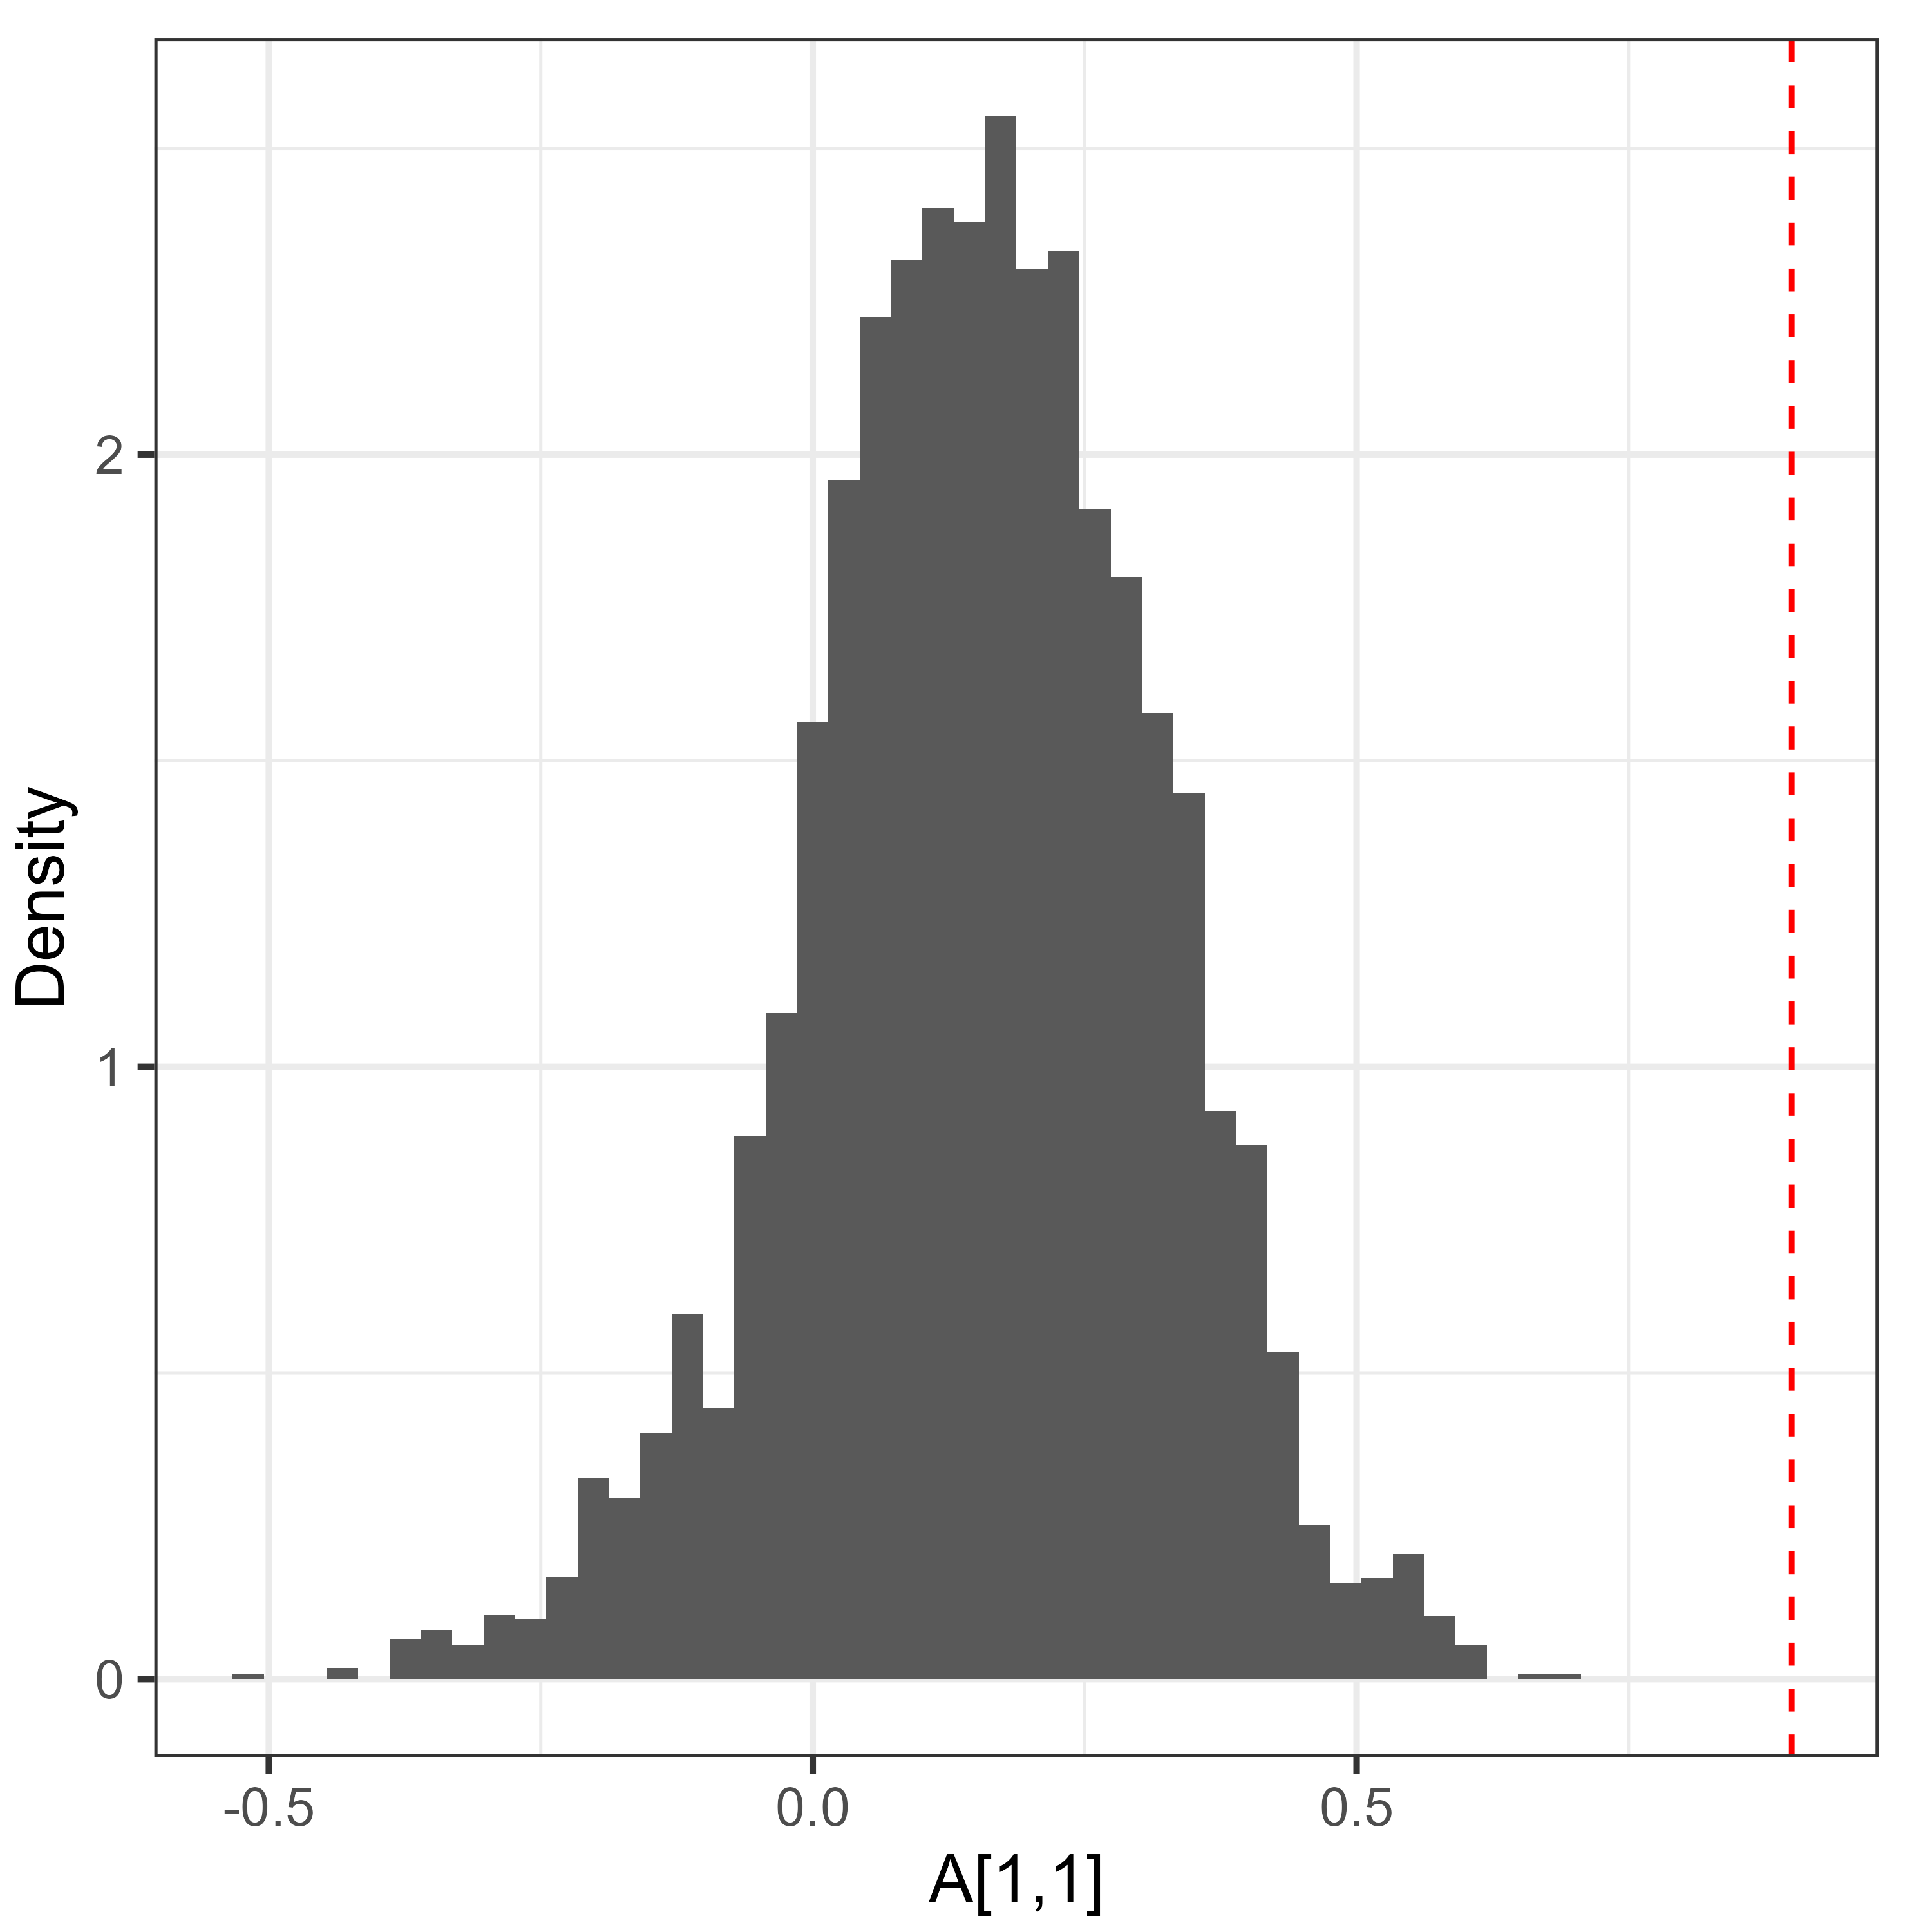
\includegraphics[width=0.32\textwidth]{../figures/post_A11.png}
    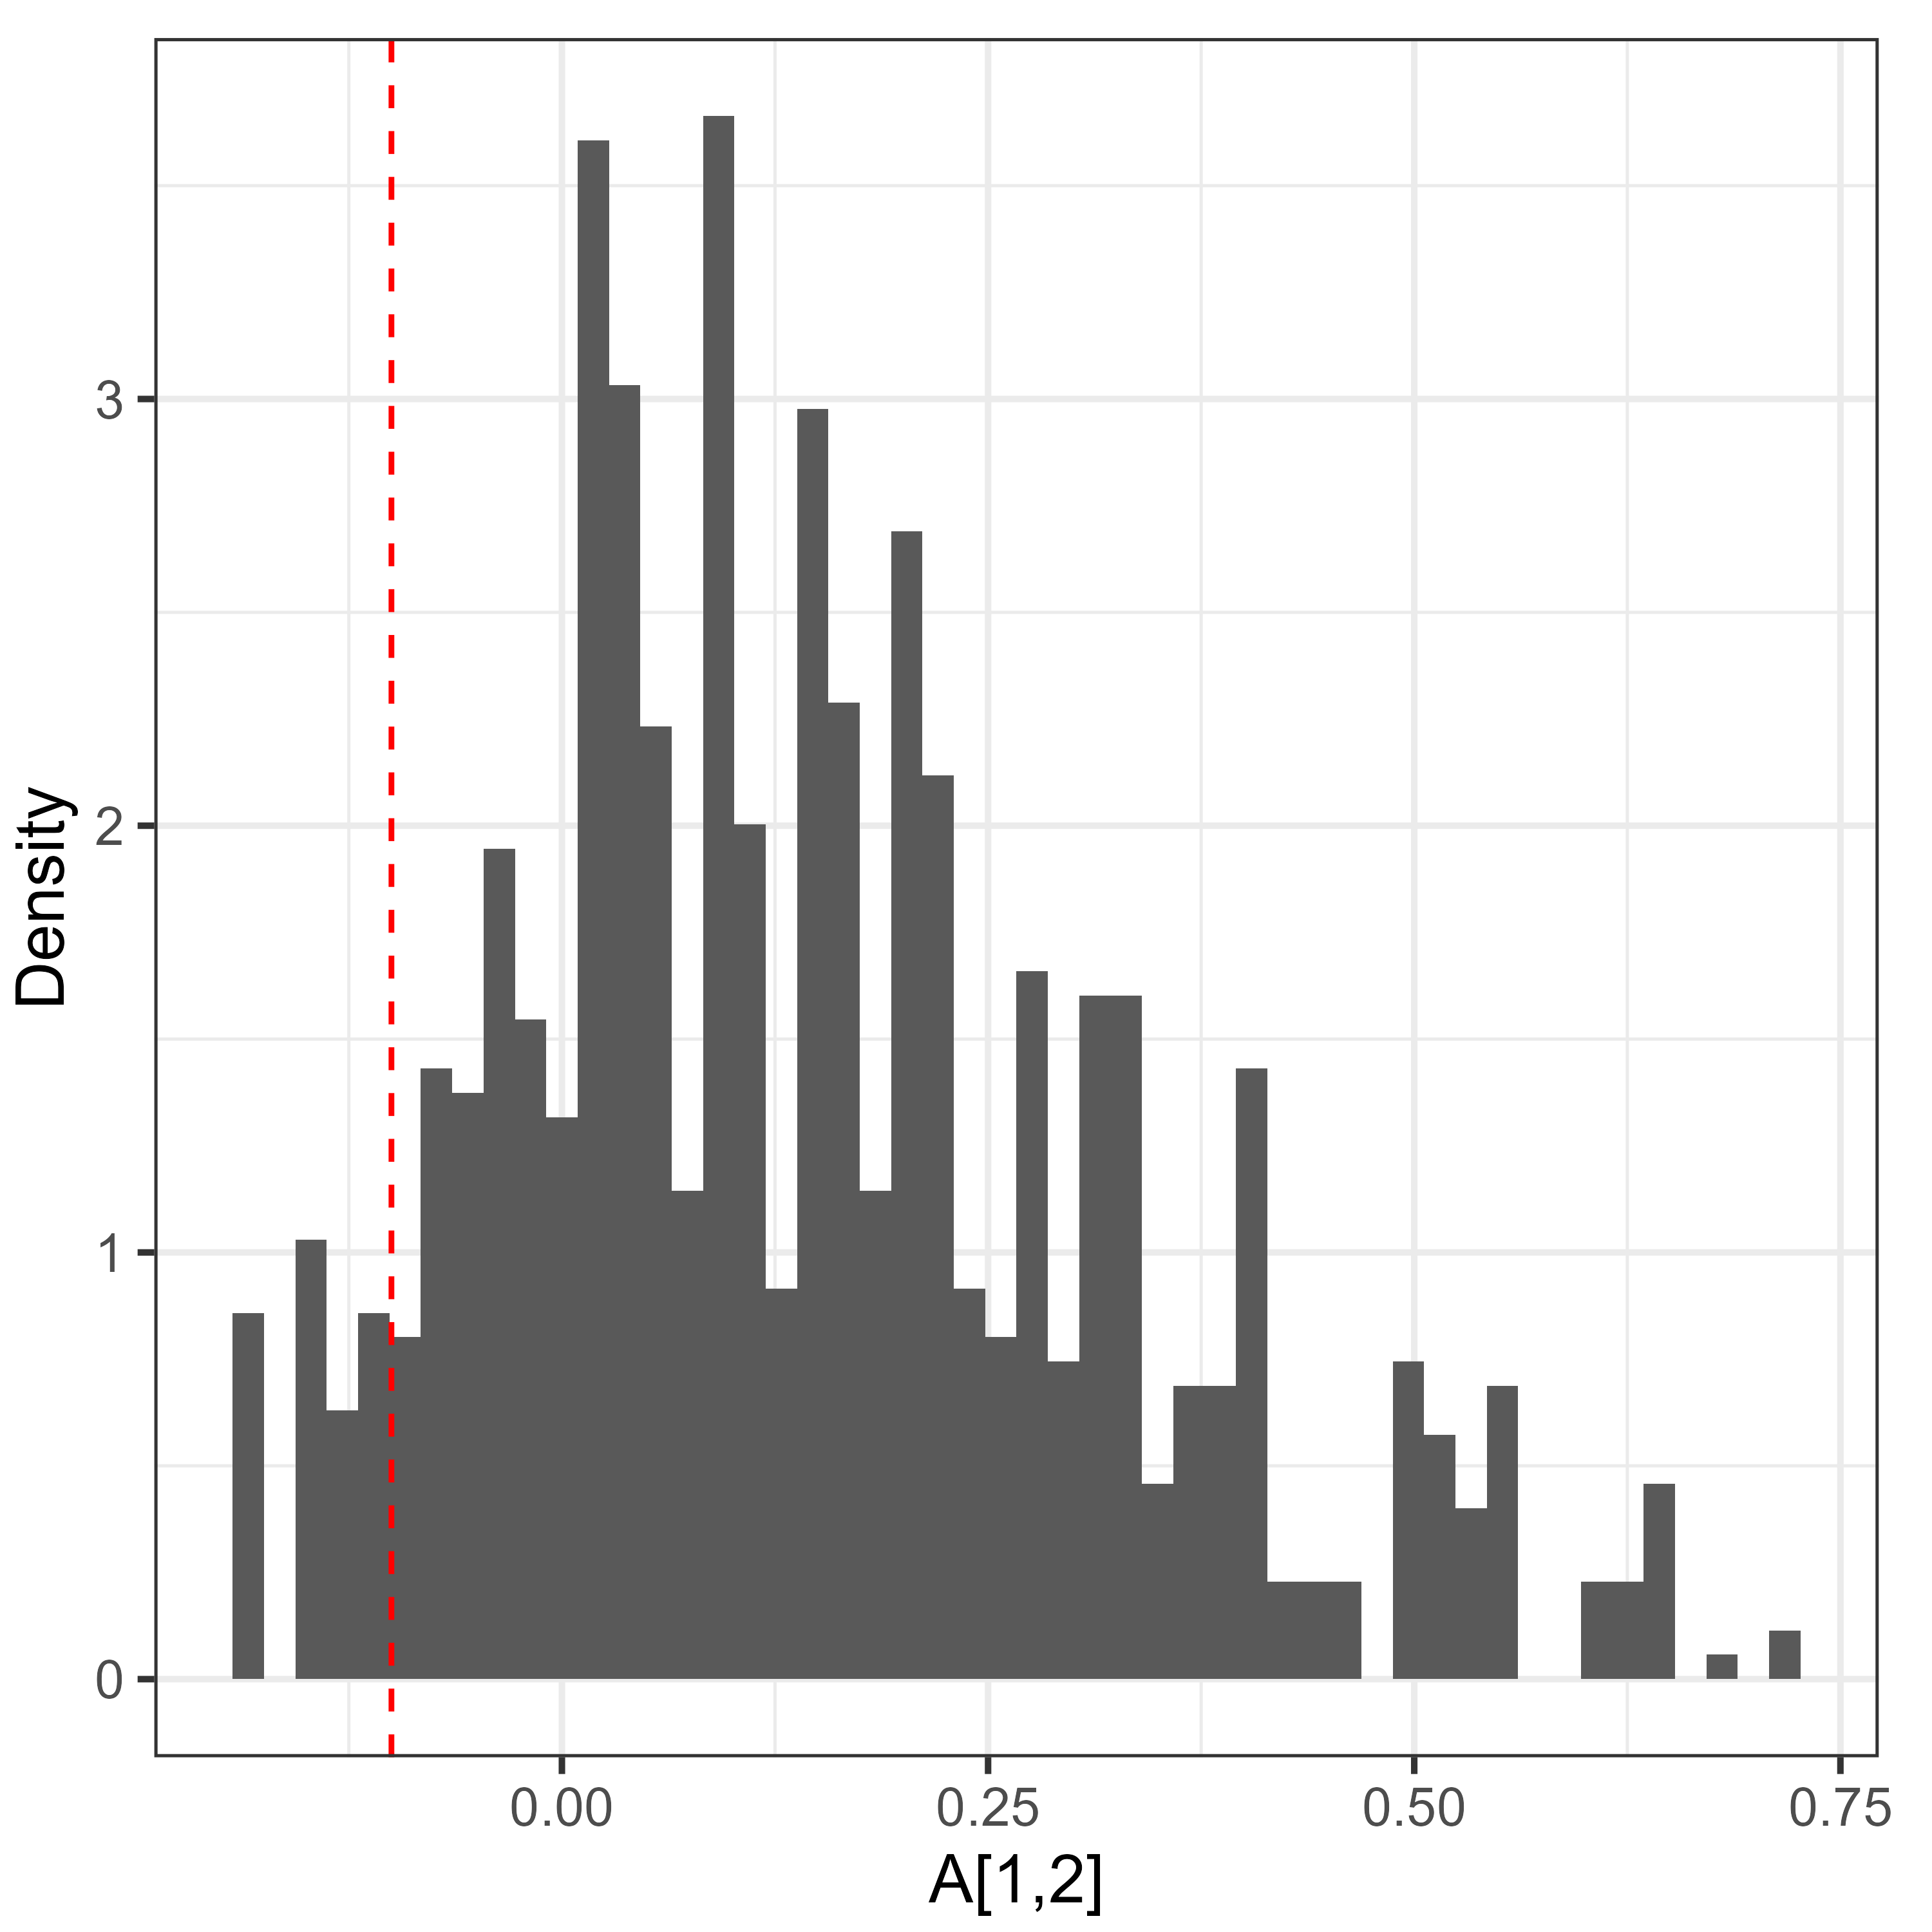
\includegraphics[width=0.32\textwidth]{../figures/post_A12.png}
    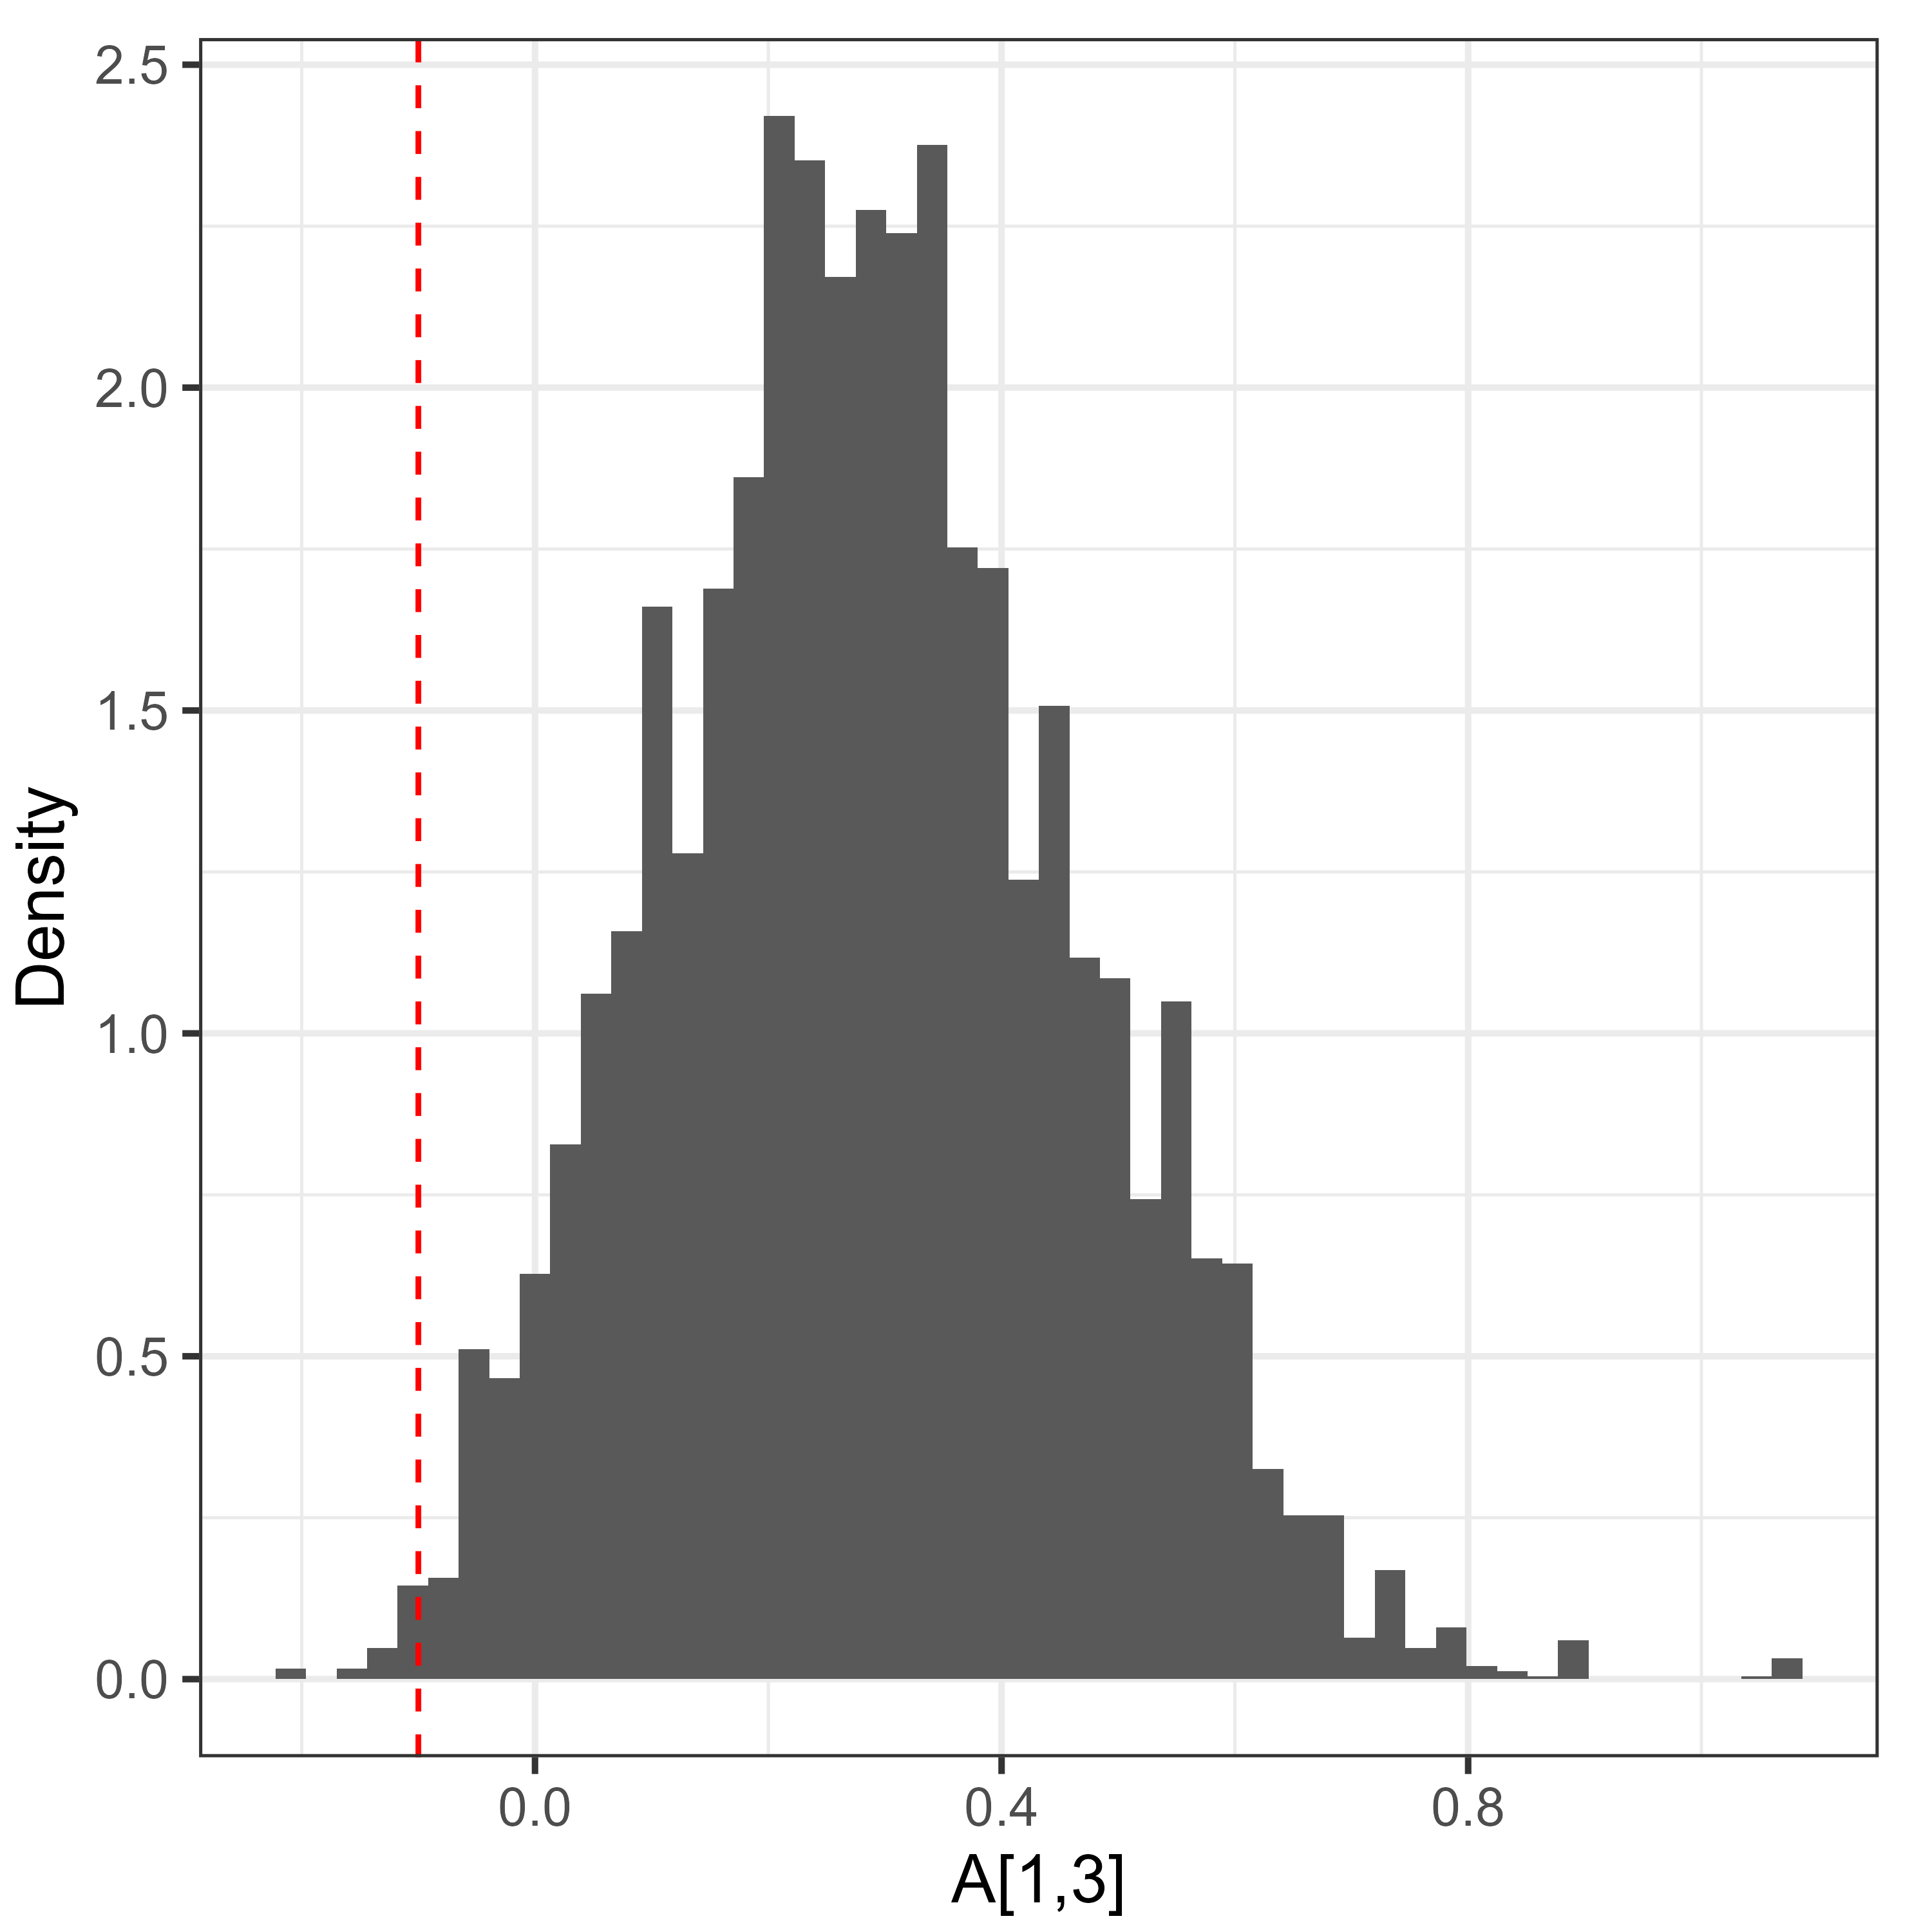
\includegraphics[width=0.32\textwidth]{../figures/post_A13.png}
    
    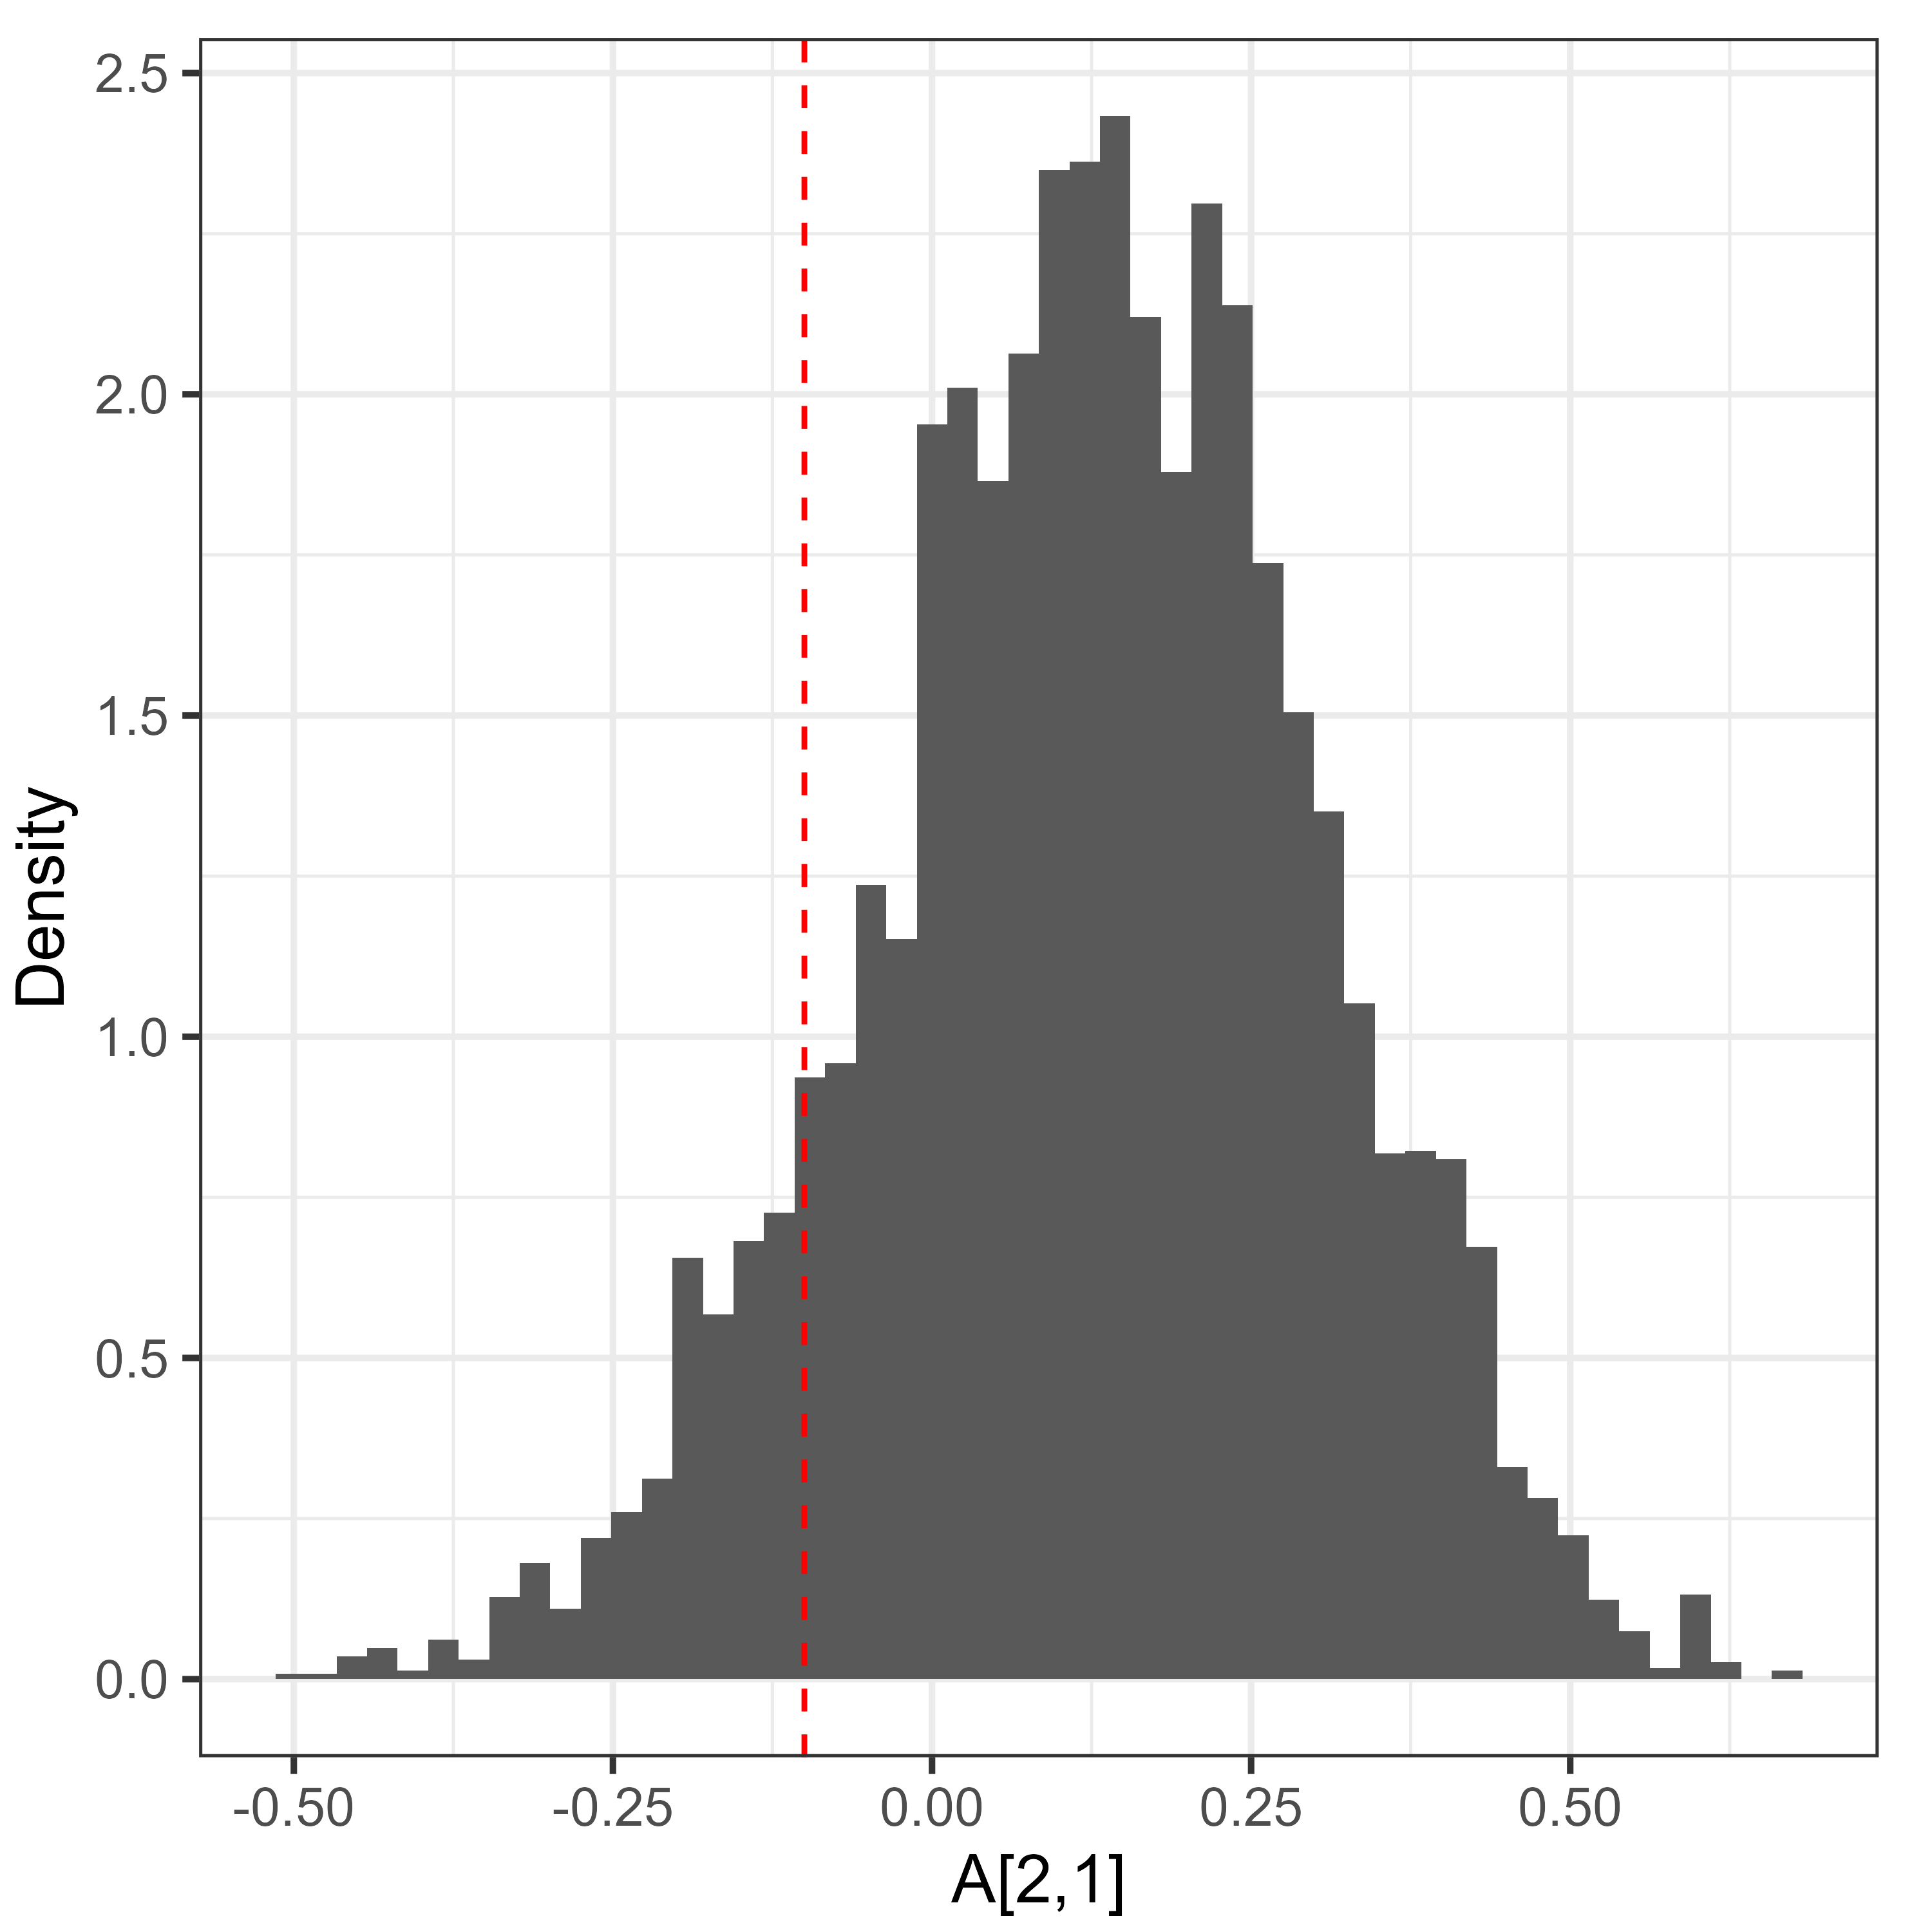
\includegraphics[width=0.32\textwidth]{../figures/post_A21.png}
    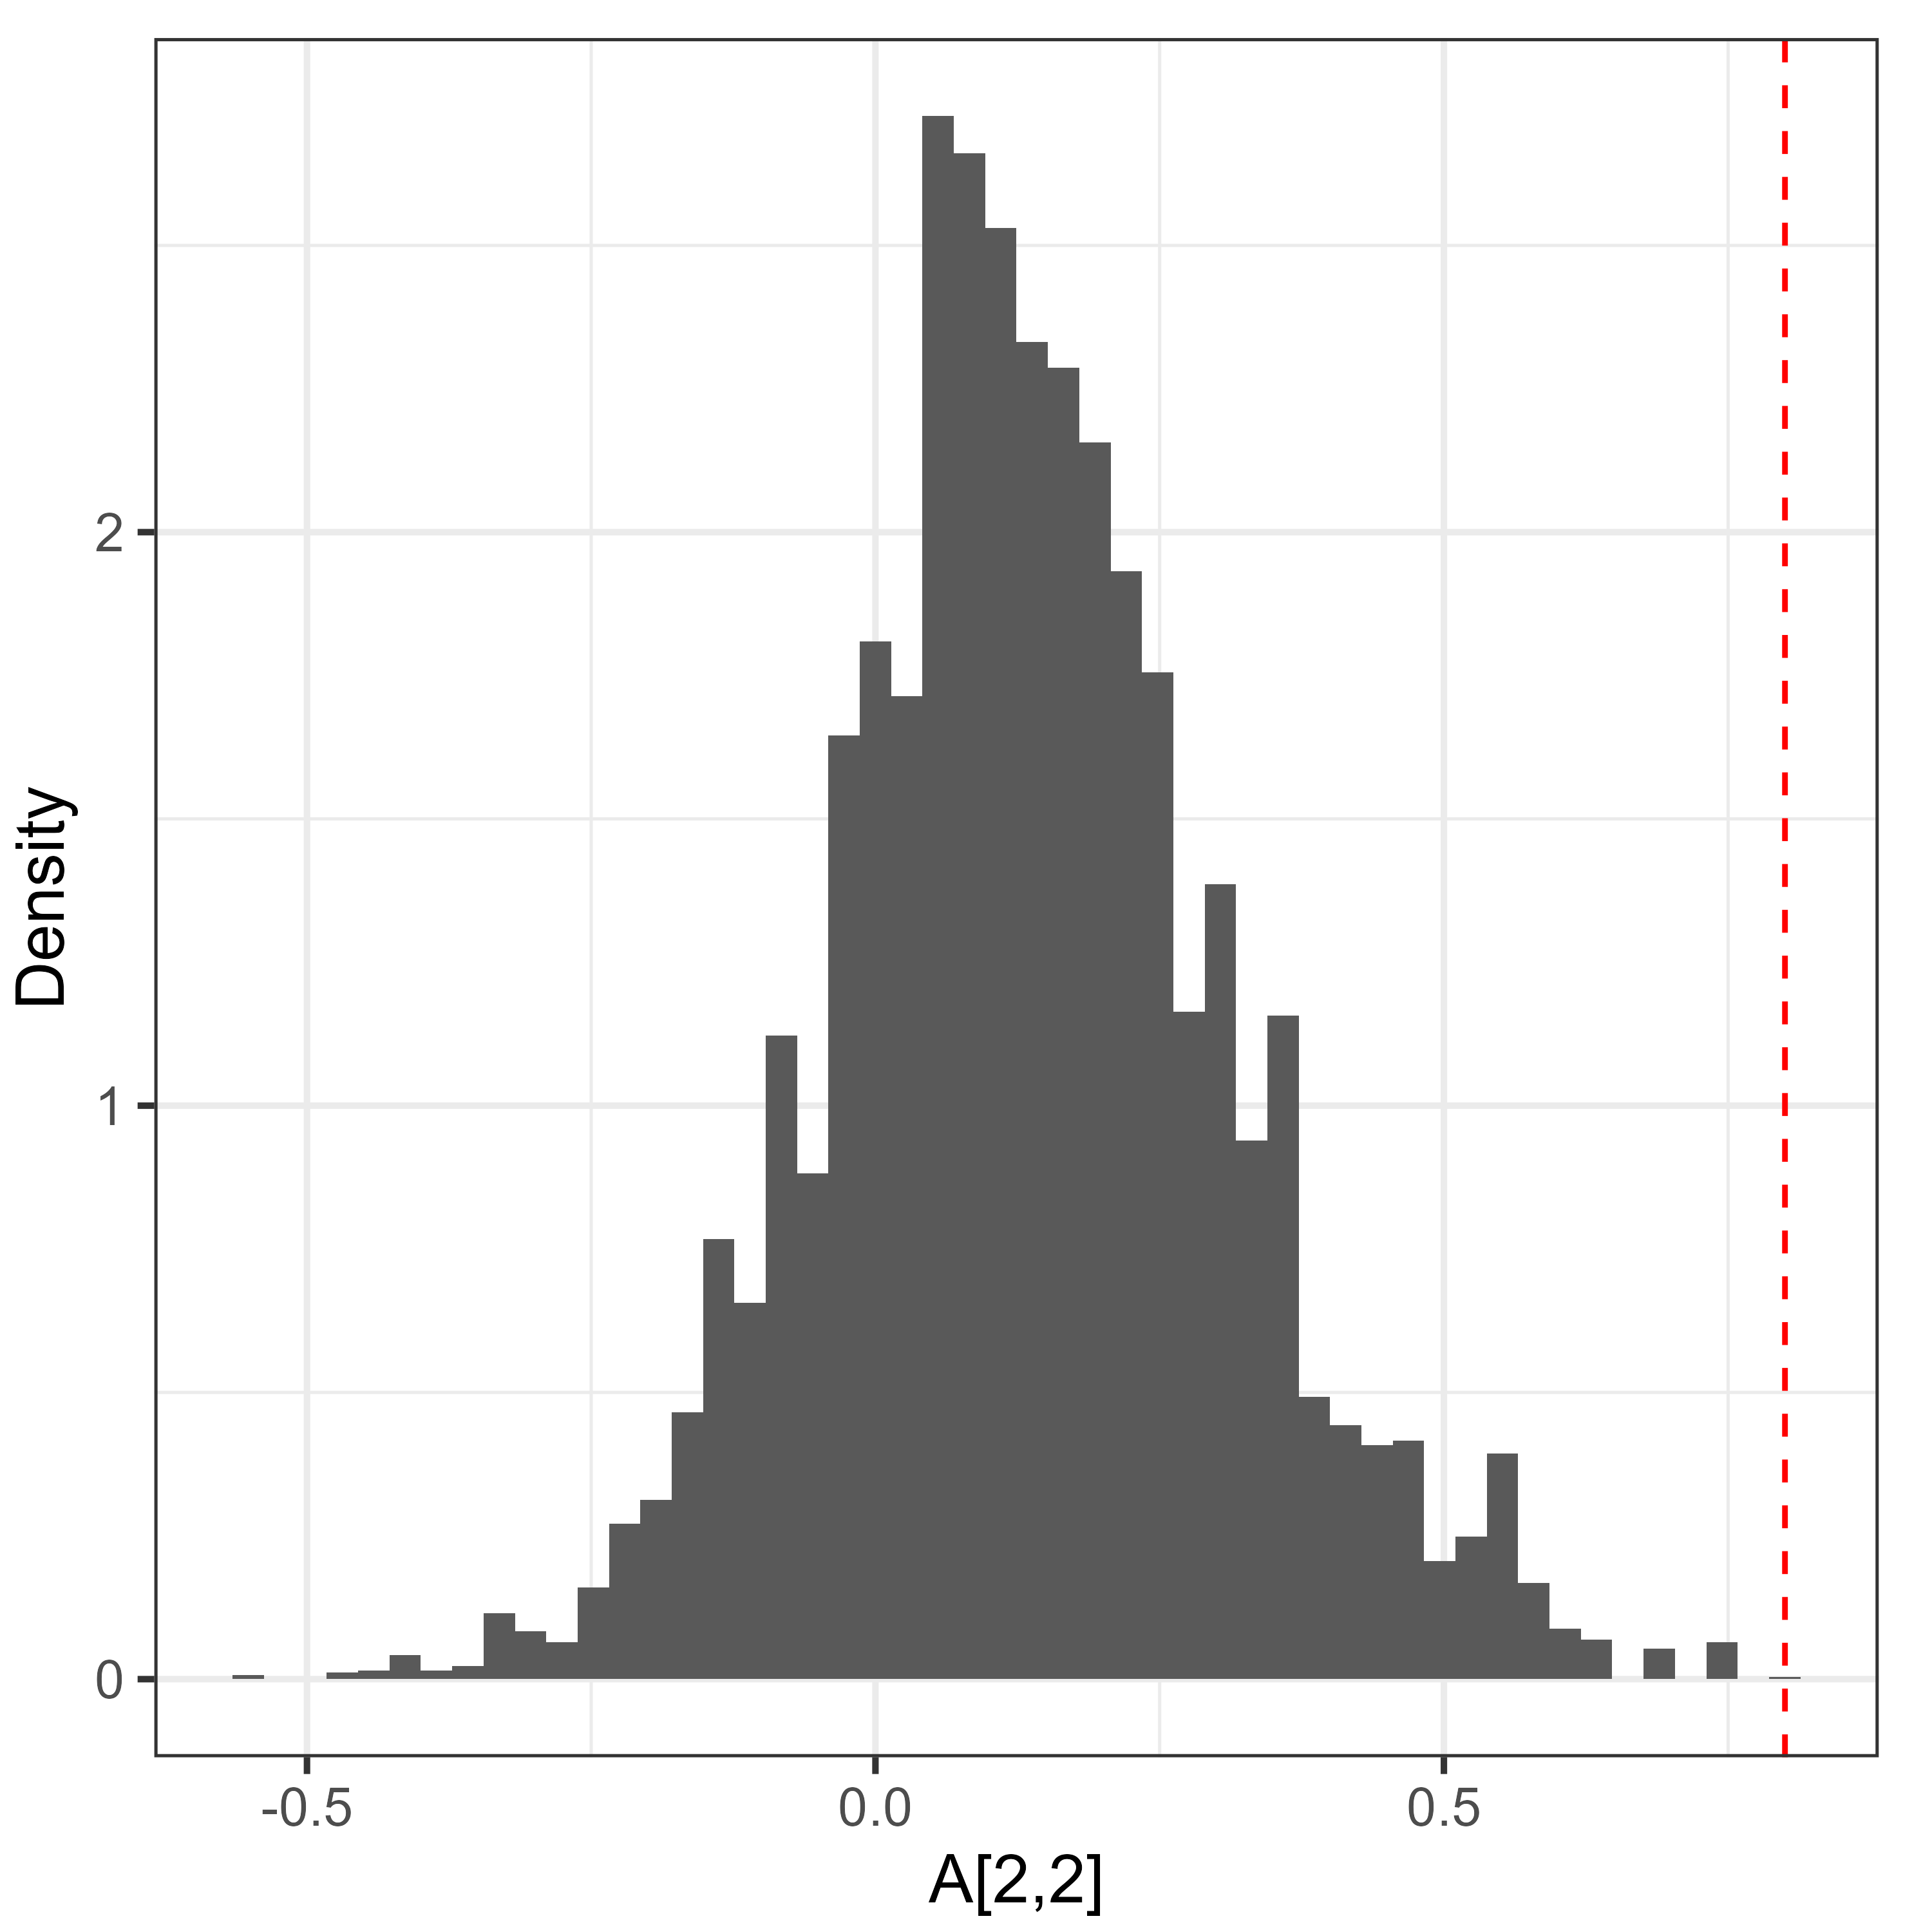
\includegraphics[width=0.32\textwidth]{../figures/post_A22.png}
    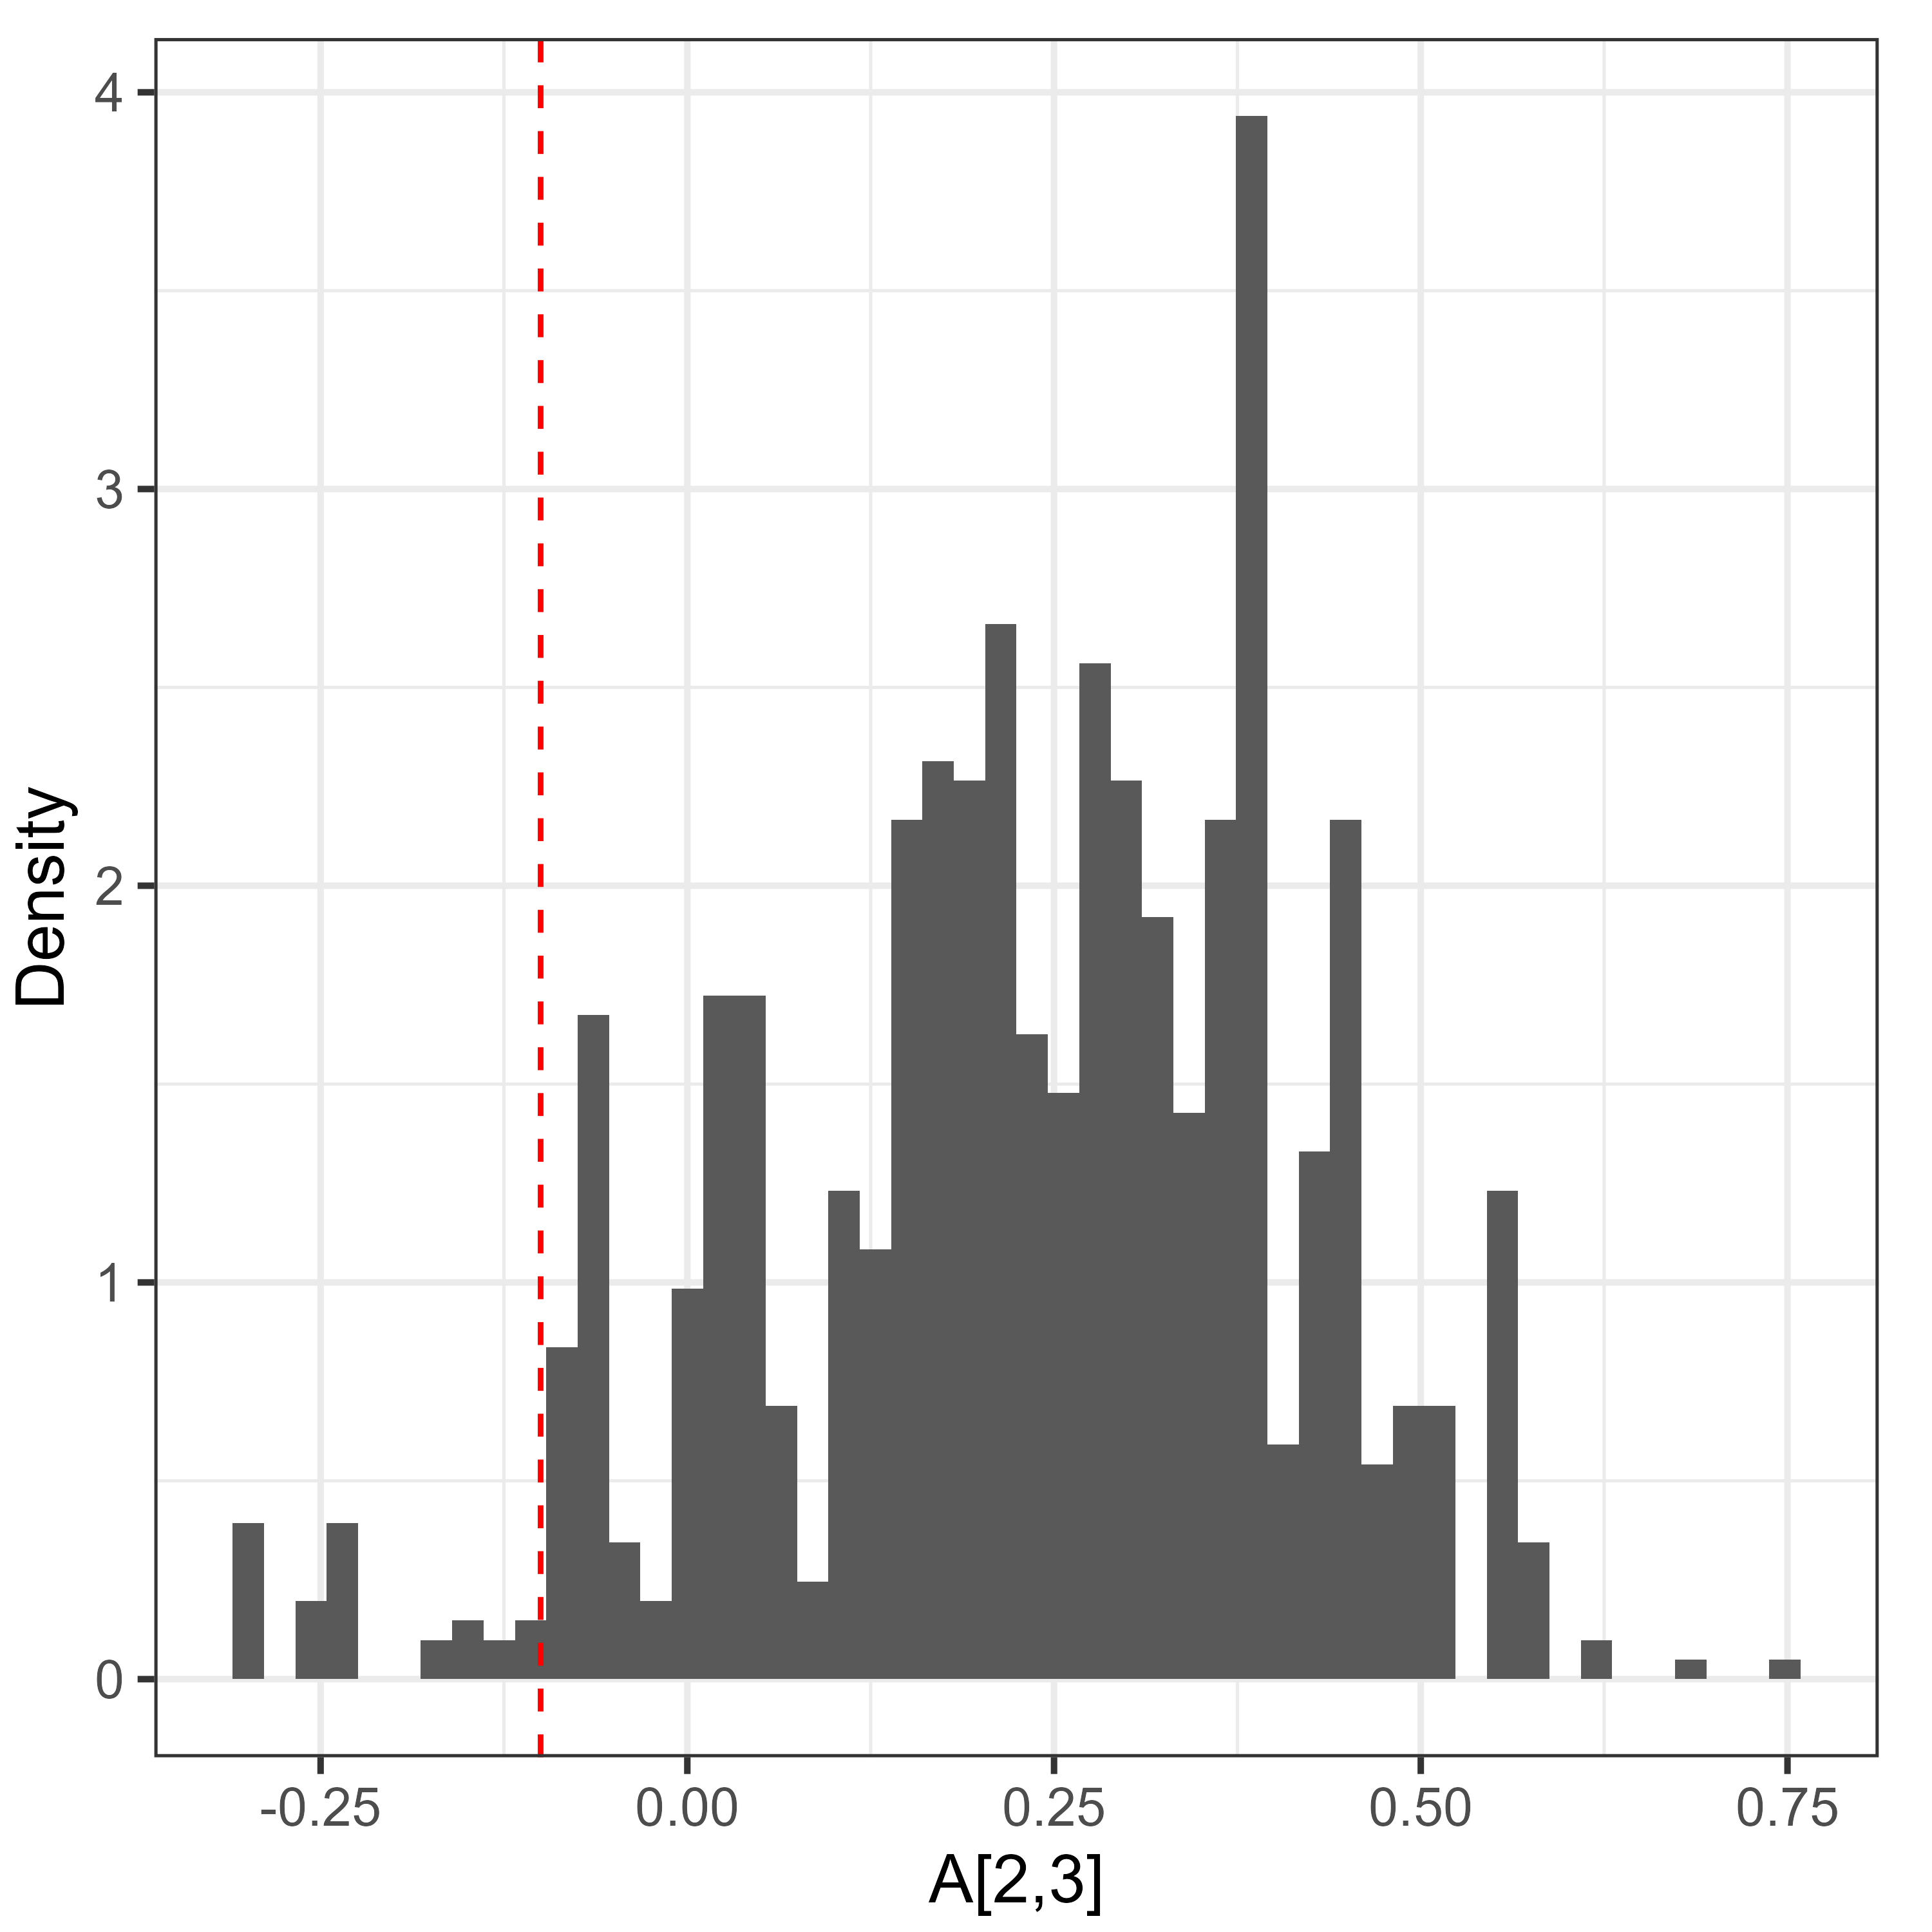
\includegraphics[width=0.32\textwidth]{../figures/post_A23.png}
    
    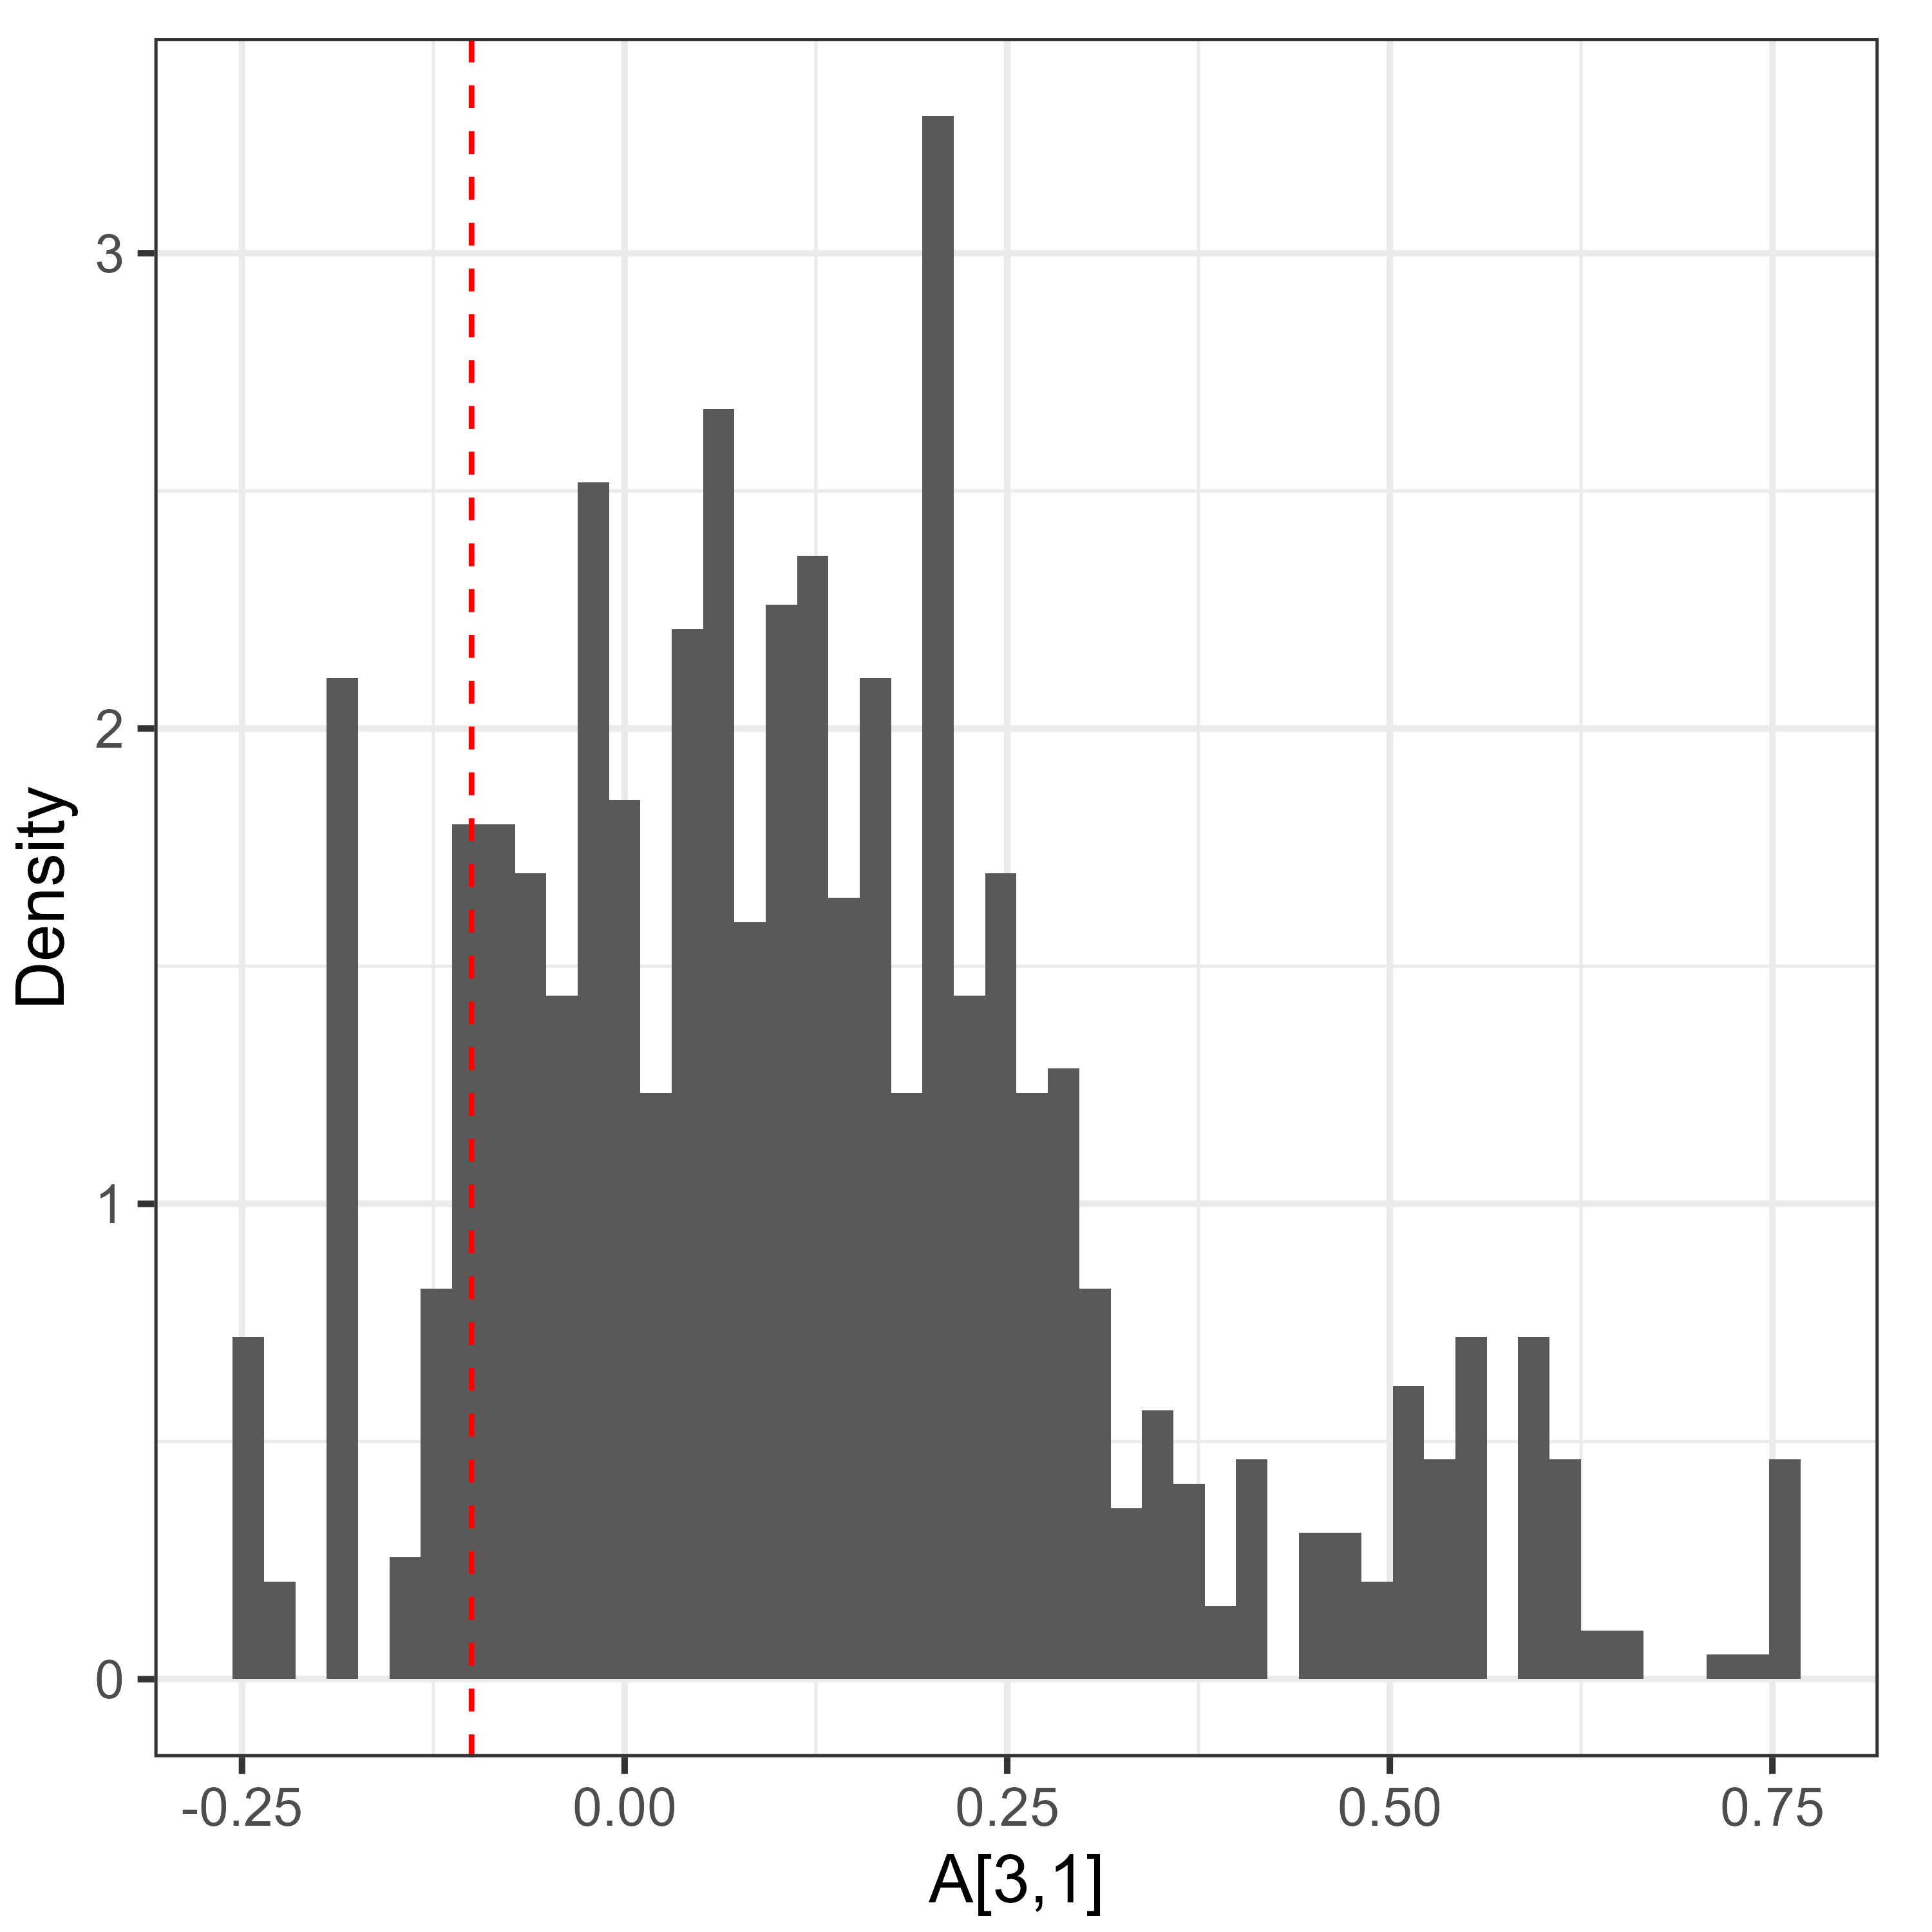
\includegraphics[width=0.32\textwidth]{../figures/post_A31.png}
    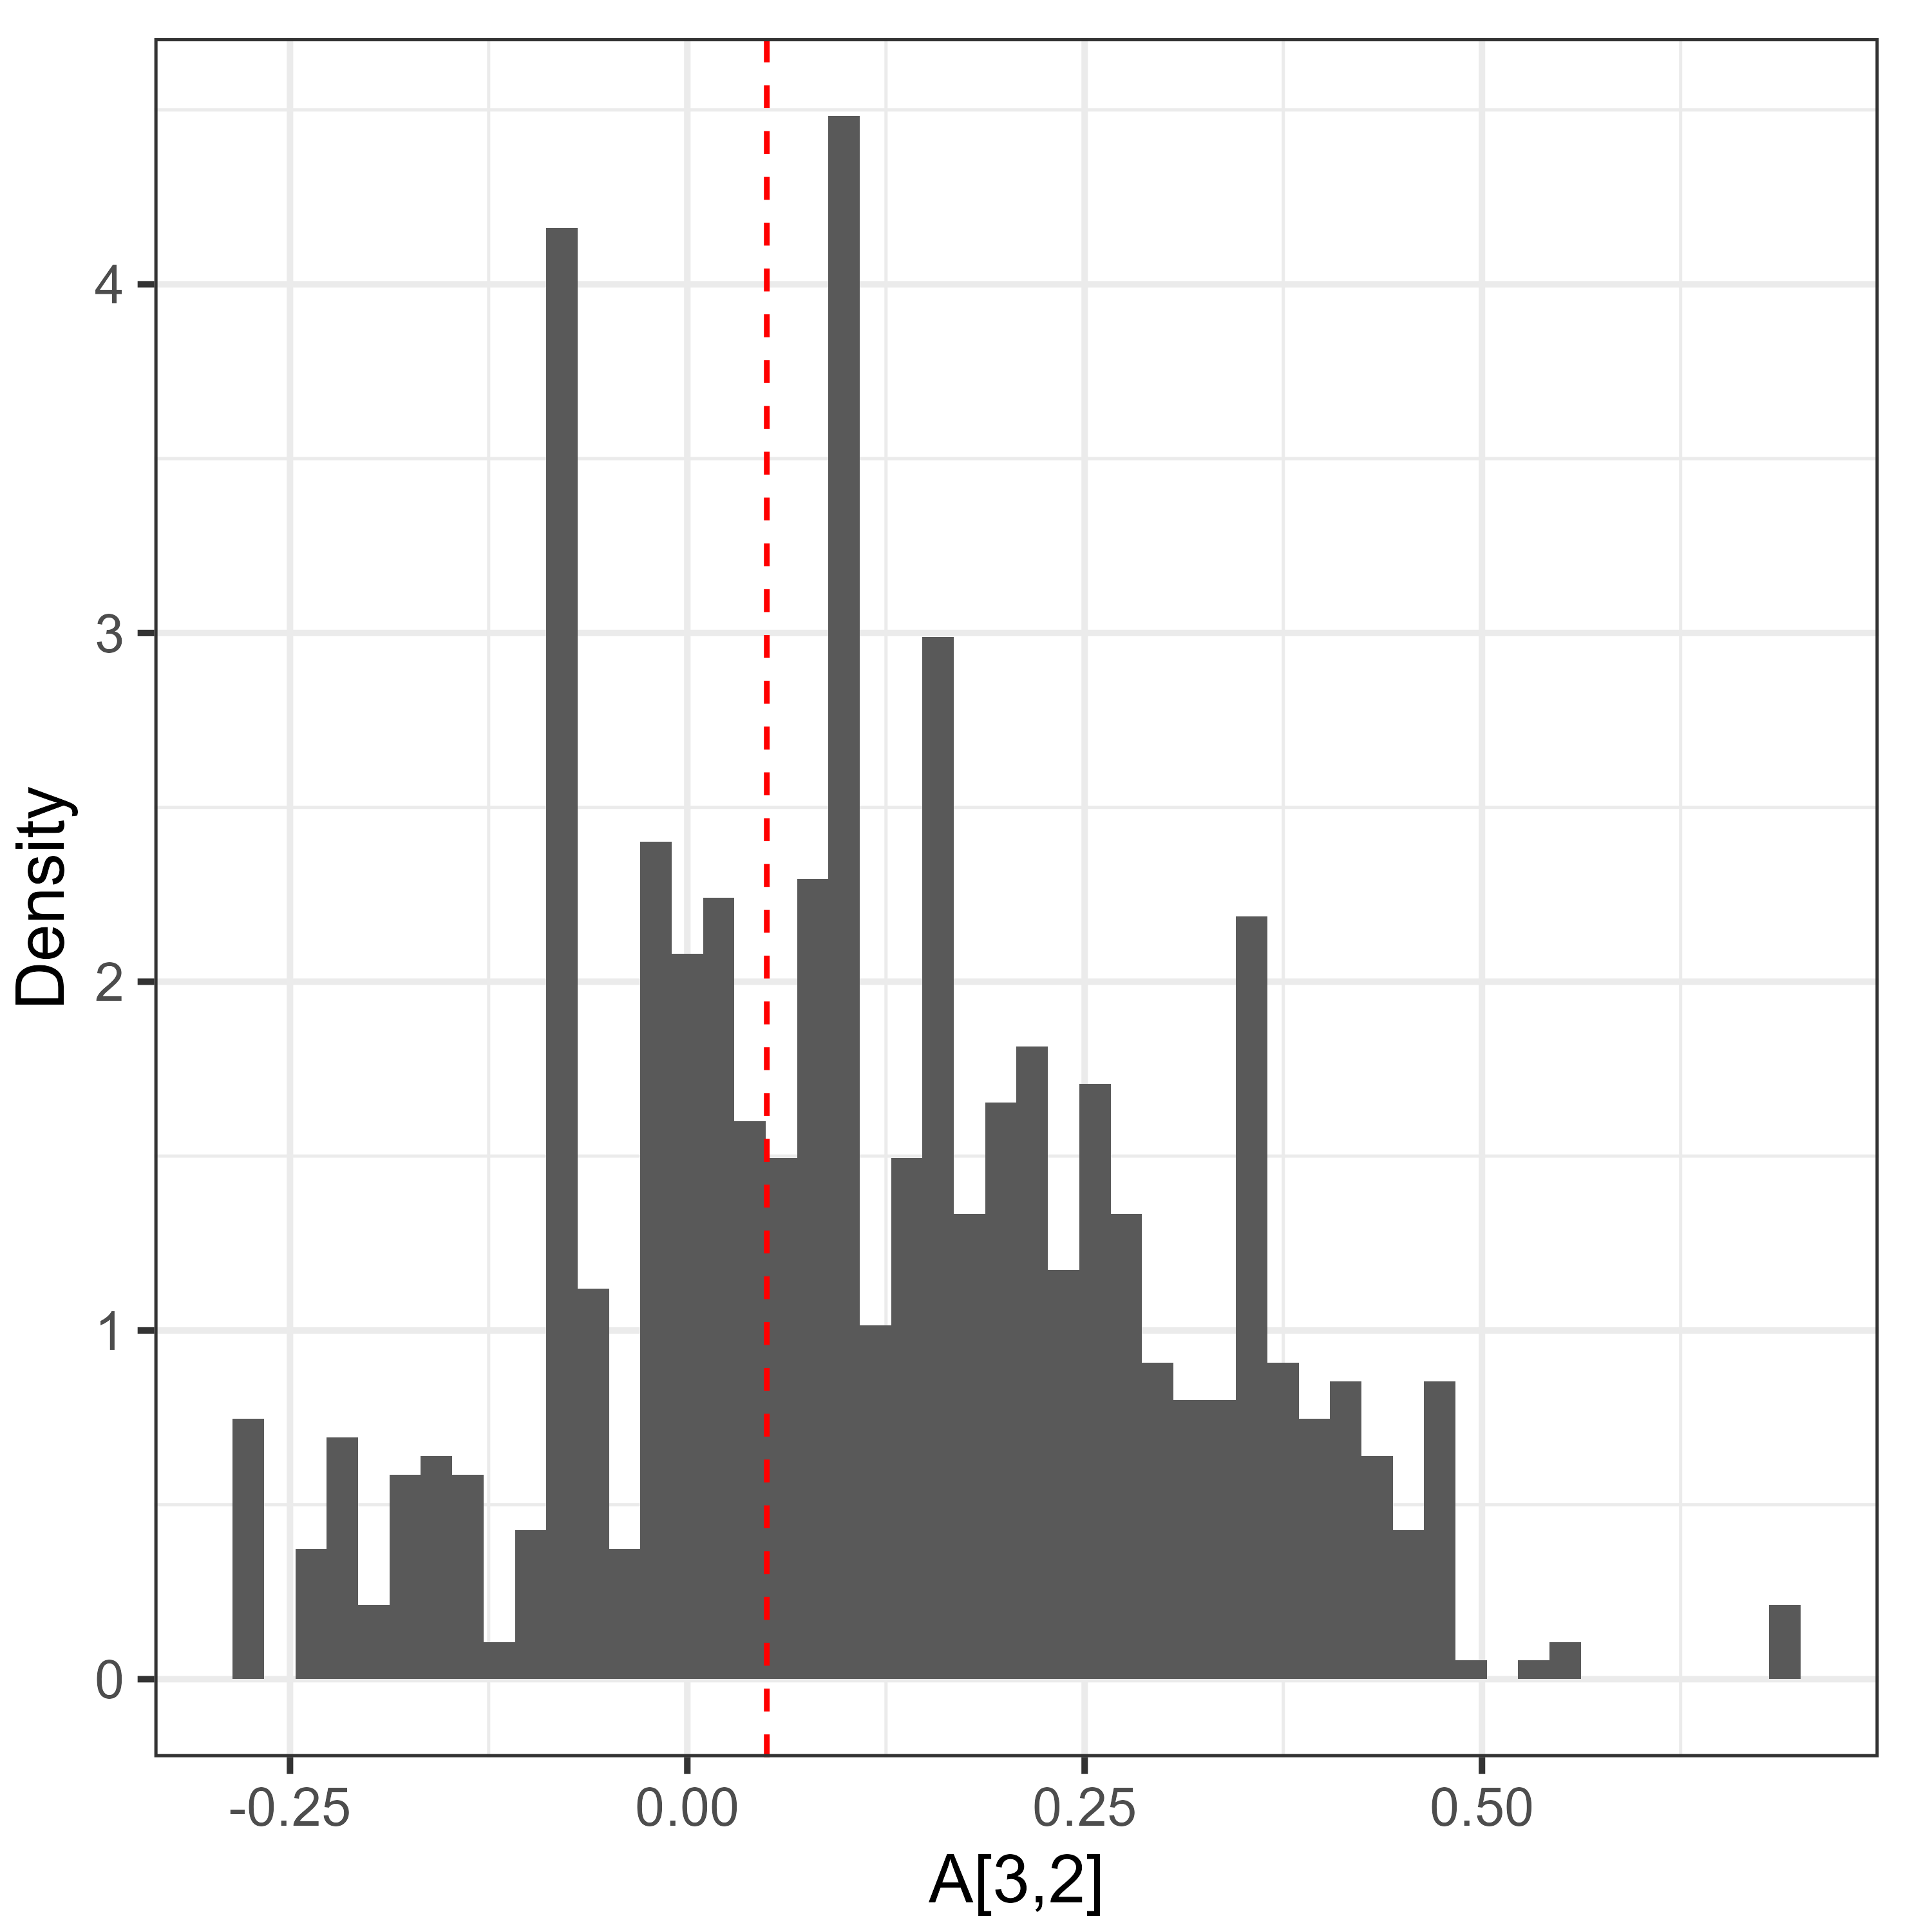
\includegraphics[width=0.32\textwidth]{../figures/post_A32.png}
    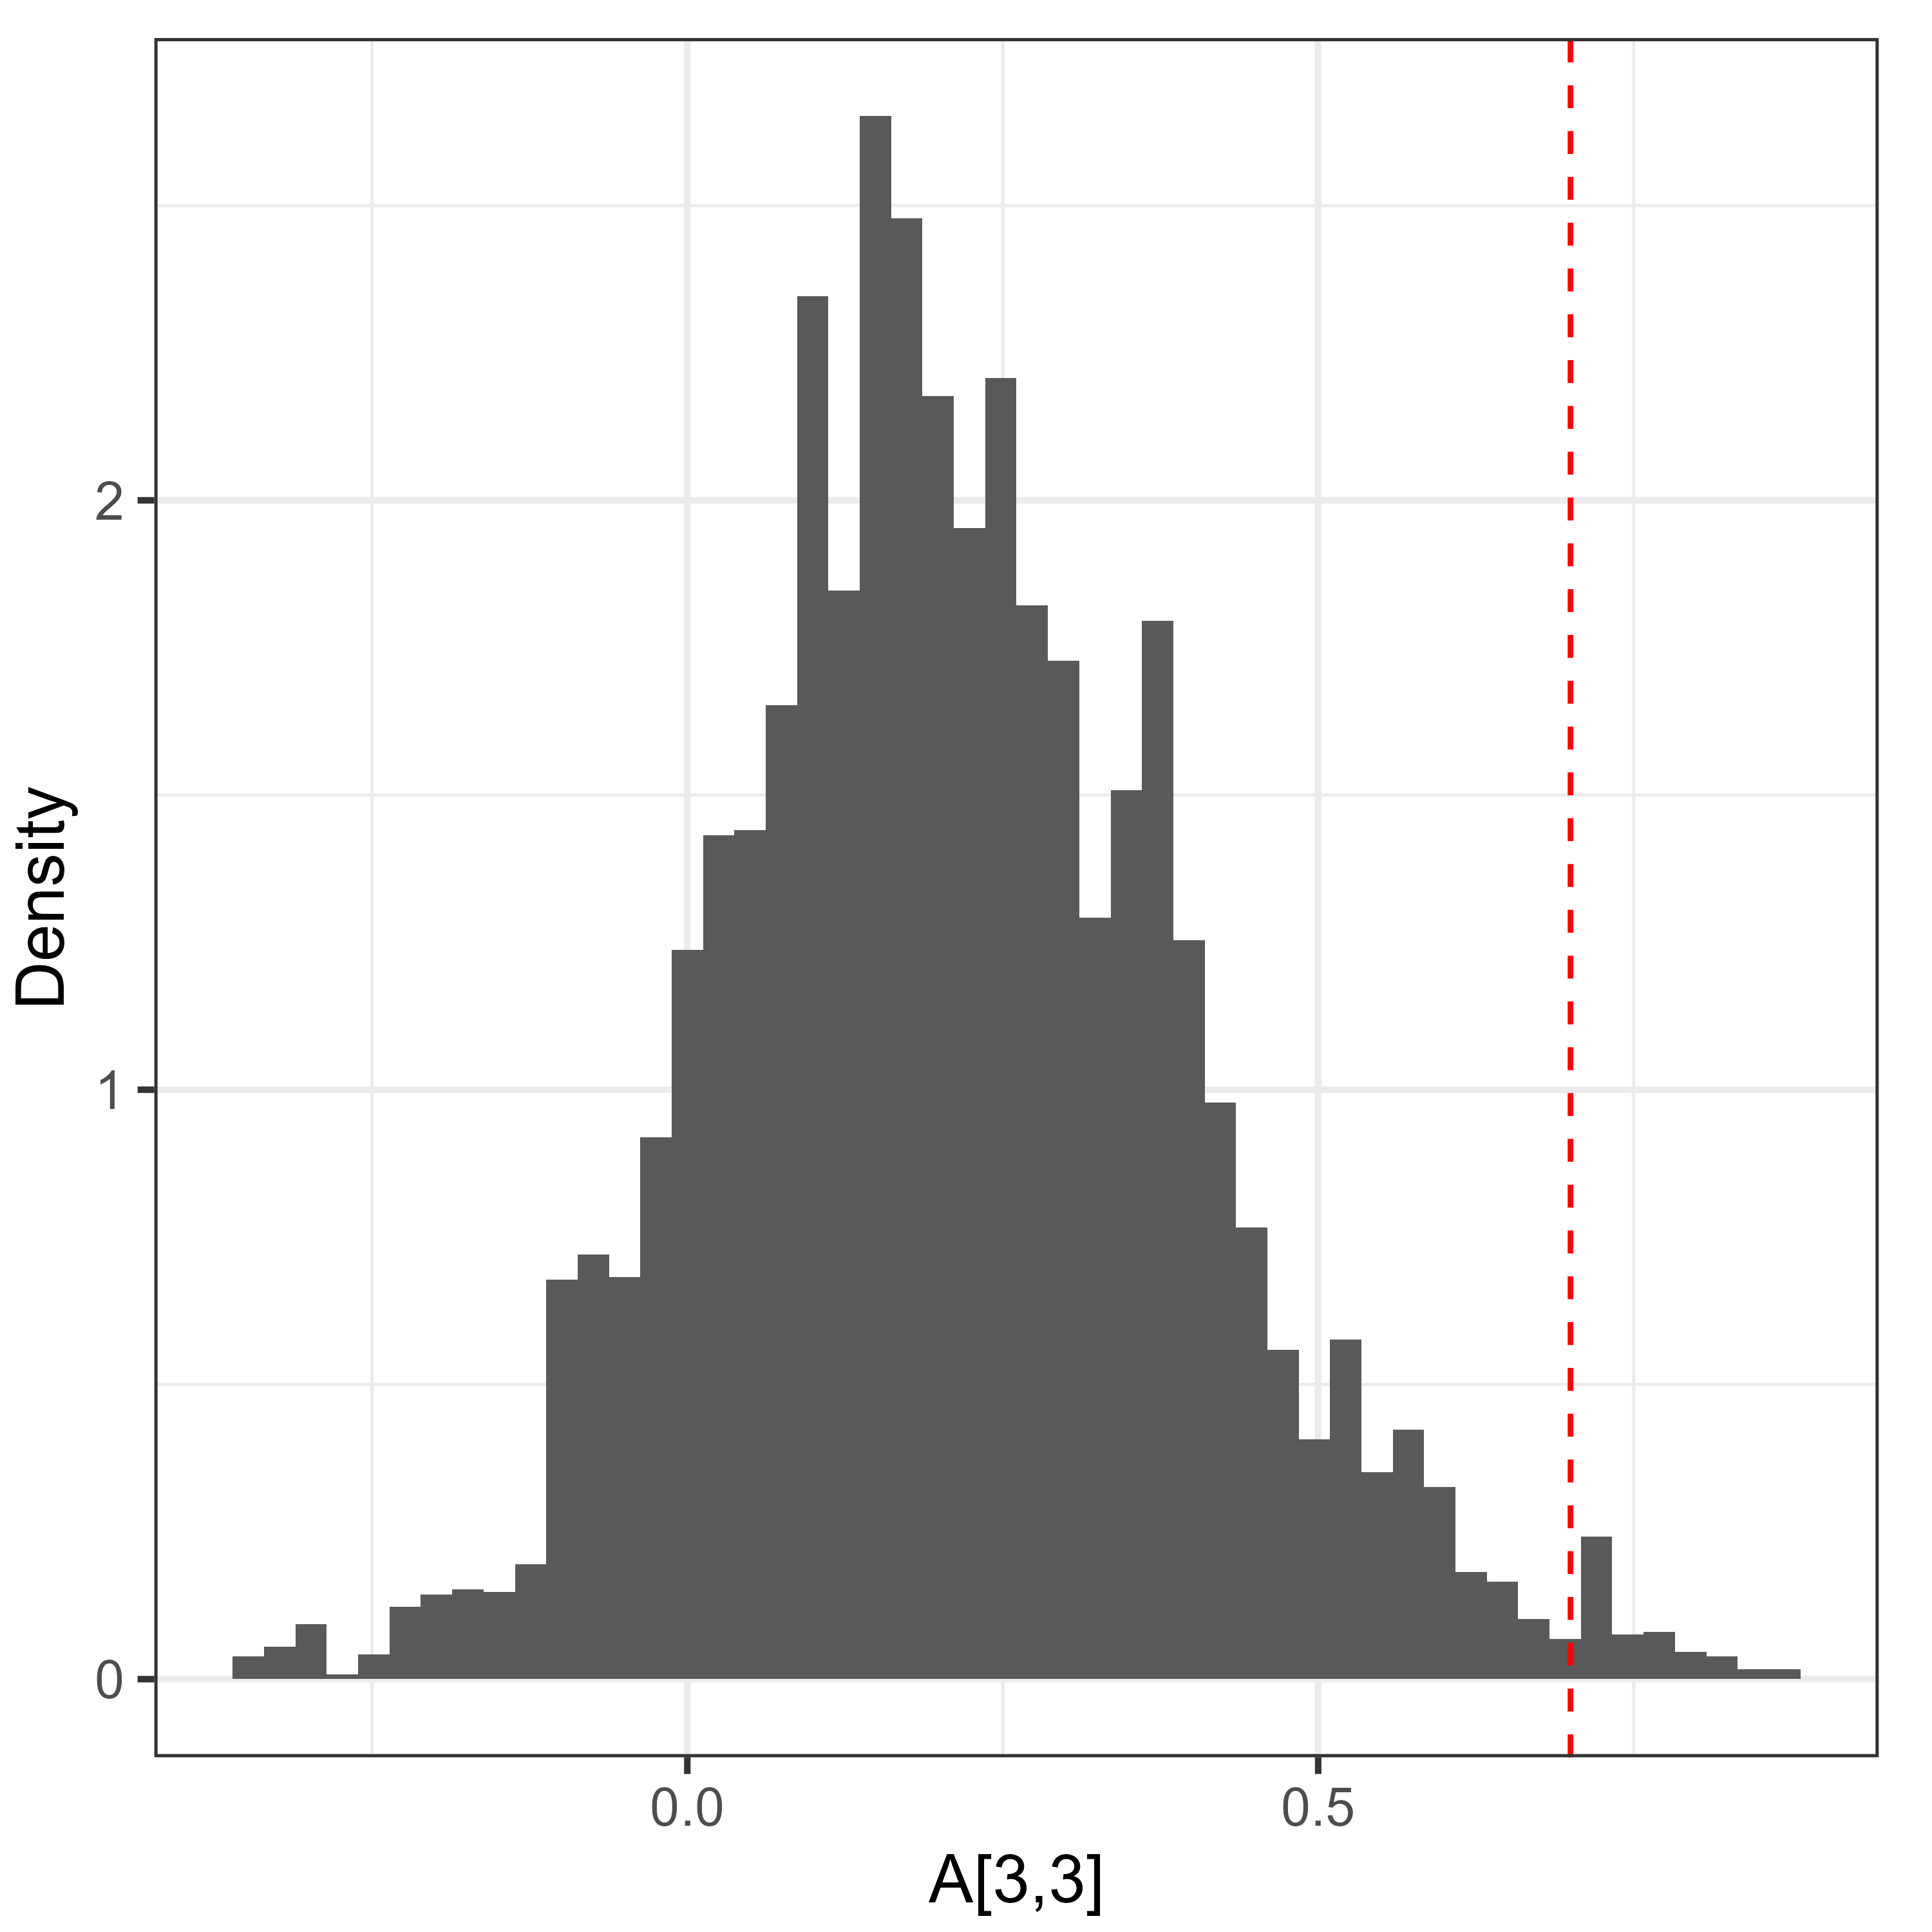
\includegraphics[width=0.32\textwidth]{../figures/post_A33.png}
    \caption{Posterior densities for the elements of $\mathbf{A}$.}
\end{figure}